\section{Theoretische Grundlagen}

\subsection{Tunneleffekt}
Bei der Rastertunnelmikroskopie tastet eine leitende Sonde mit dünner Spitze eine Probe ab. Das Vakuum (bzw. die Luft) zwischen Spitze und Probe stellt für Elektronen aus der Spitze eine Potentialbarriere dar, da sie sich in der Spitze in einem gebundenen Zustand befinden. Klassisch könnte kein Strom zwischen Spitze und Probe fließen wenn die gebundenen Elektronen eine Energie $E$ kleiner als die Potentialbarriere haben. Quantenmechanisch kann durch den Tunneleffekt jedoch ein Strom fließen. Um diesen Effekt zu verstehen wird die Potentialbarriere stark vereinfacht als ein Kastenpotential mit Höhe $V_0>0$ betrachtet (siehe Abbildung \ref{fig:tunnel}). Außerdem wird angenommen, dass die Elektronen in Spitze und Probe als frei betrachtet werden können. Die stationären Zustände der resultierenden Schrödingergleichung können nun leicht berechnet werden. Der Transmissionswahrscheinlichkeit $T$ für eine von der Spitze zur Probe laufende Materiewelle ist dann gegeben durch
\begin{align*}
  \frac{1}{T}=1+\frac{1}{4}\left( 2+\frac{E}{V_0-E} + \frac{V_0-E}{E}\right) \sinh^2\left( 2a \frac{\sqrt{2m(V_0-E)}}{\hbar} \right), 
\end{align*}
wobei $m$ die Elektronenmasse, $\hbar$ das Plancksche Wirkungsquantum und $a$ die Ausdehnung des Potentials ist.
Für große Argumente des $\sinh$ folgt also
\begin{align}
  T \propto e^{-4a\sqrt{2m(V_0-E)}/\hbar}.
  \label{eq:T}
\end{align}  
Der Tunnelstrom hängt also stark von dem Abstand $a$ ab. Genau diese starke Abhängigkeit wird bei der Rastertunnelmikroskopie ausgenutzt. 


\begin{figure}[h]
  \centering
  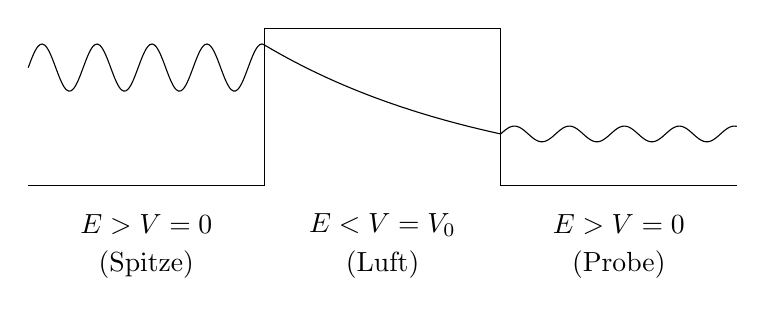
\begin{tikzpicture}
    \draw (0,0)--(3,0)--(3,2)--(6,2)--(6,0)--(9,0);
    \draw (1.5,-0.5) node {$E>V=0$};
    \draw (1.5,-1) node {(Spitze)};
    \draw (4.5,-0.5) node {$E<V=V_0$};
    \draw (4.5,-1) node {(Luft)};
    \draw (7.5,-0.5) node {$E>V=0$};
    \draw (7.5,-1) node {(Probe)};
    \draw [smooth,samples=100,domain=0:3] plot (\x,{1.5+0.3*sin(9*\x r)});
    \draw [smooth,samples=100,domain=3:6] plot (\x,{(1.5+0.3*sin(9*3 r))*exp(-(\x-3)/3)});
    \draw [smooth,samples=100,domain=6:9] plot (\x,{(1.5+0.3*sin(9*3 r))*exp(-(6-3)/3)+0.1*sin(9*(\x-6) r)});
  \end{tikzpicture}
  \caption{Visualisierung des Tunneleffektes (ohne reflektierte Wellenanteile)}
  \label{fig:tunnel}
\end{figure}

\subsection{Funktionsweise des RTM}
Der grobe Aufbau eines RTM ist in Abbildung \ref{fig:RTM} zu sehen und wird in \cite{RWTH} detailliert erklärt. Durch das Anlegen einer Spannung $U$ zwischen Spitze und Probe können die Fermi-Niveaus beider Materialien so gegeneinander verschoben werden, dass ein Netto-Elektronenfluss von Spitze zu Probe (oder andersherum) enstehen kann. 
Man unterscheidet zwischen zwei Messmethoden, der \textit{constant current method} (CCM) und der \textit{constant height method} (CHM). 
\begin{figure}[h]
  \centering
  \begin{tikzpicture}
     \draw [pattern=north west lines] (3.5,2.5) -- (3.75,1) -- (4,2.5) -- cycle;
     \foreach \x  in {1.5,2,2.5,3,3.5,4}%
        \draw  (1+\x,0.8) circle (0.15cm);
     \foreach \x  in {1.5,2,2.5,3,3.5,4}%
        \draw  (0.75+\x,0.6) circle (0.15cm);
     \foreach \x  in {1.5,2,2.5,3,3.5,4}%
        \draw  (0.5+\x,0.4) circle (0.15cm);
     \foreach \x  in {1.5,2,2.5,3,3.5,4}%
        \draw  (0.25+\x,0.2) circle (0.15cm);
      \foreach \x  in {1.5,2,2.5,3,3.5,4}%
        \draw  (\x,0) circle (0.15cm);
      \draw (4,-0.15) -- (4,-0.5) -- (6,-0.5) -- (6,0);
      \draw (6,0.2) circle (0.2cm);
      \draw [->] (5.7,-0.1) -- (6.3,0.5);
      \draw (6,0.4) -- (6,1) -- (5.9,1) -- (6.1,1);
      \draw (5.8,1.2) -- (6.2,1.2) -- (6,1.2) -- (6,2) -- (3.91,2);
      \draw (0.7,0) node {Probe};
      \draw (2.5,2) node {Spitze};
      \draw (6.4,0.2) node {$I$};
      \draw (6.4,1.1) node {$U$};
      \draw (3.25,2.5) rectangle (4.25,3);
      \draw (2,2.75) node {Piezoelement};
      \draw (6.6,0.2) -- (7.5,0.2);
      \draw [->] (7.5,0.2) -- (7.5,2.5);
      \draw (7,2.5) rectangle (8,3);
      \draw (7.5,3.25) node {Regler};
      \draw [->] (7,2.75) -- (4.25,2.75);
      \draw (5.6,3) node {$x$, $y$, $z(I)$};
      \draw [->] (8,2.75) -- (9,2.75);
      \draw (9.5,2.75) node {Bild};
      \draw [->] (-1.5,0) -- (-2.1,-0.6);
      \draw [->] (-1.5,0) -- (-0.5,0);
      \draw [->] (-1.5,0) -- (-1.5,1);
      \draw (-1.7,1) node {$z$};
      \draw (-2.3,-0.6) node {$x$};
      \draw (-0.3,0) node {$y$};
  \end{tikzpicture}
  \caption{Schematischer Aufbau des RTM}
  \label{fig:RTM}
\end{figure}

\subsubsection{Piezoelektrizität}
Die Spitze des Rastertunnelmikroskops muss für die Untersuchung von Materialien sehr präzise bewegt werden. Dies wird mit Piezoelementen erreicht. Piezoelektrische Materialien haben die Eigenschaft, dass sie sich durch das Anlegen einer Spannung verformen und andersherum auch durch Verformung eine Spannung induzieren. Verstanden werden kann dieses Prinzip durch Betrachtung einer Elementarzelle mit 6 Ladungen (siehe Abbildung \ref{fig:piezo}). Im Grundzustand liegen die Ladungsschwerpunkte in der Mitte der Zelle und somit verschwindet das Dipolmoment. Durch Stauchung liegt der positive über dem negativen Ladungschwerpunkt und ein Dipolmoment entsteht. Makroskopisch kommt es auf die Anordnung der Elementarzellen an und der Effekt wird deutlich komplizierter. Für größere Längenänderungen werden z.B. mehrere Piezoelemente zu einem Piezoaktor zusammengeschlossen.

\begin{figure}[h]
  \centering
  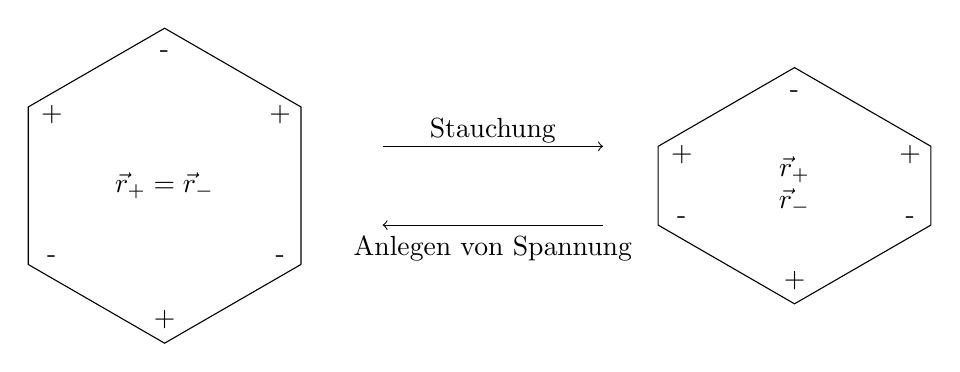
\begin{tikzpicture}
    \draw (2*1.732,0)--(2*0.866,-2*0.5)--(0,0)--(0,2*1)--(2*0.866,2*1.5)--(2*1.732,2*1)--(2*1.732,0);
    \draw (2*5.732,0+0.5)--(2*4.866,-2*0.5+0.5)--(2*4,0+0.5)--(2*4,2*1-0.5)--(2*4.866,2*1.5-0.5)--(2*5.732,2*1-0.5)--(2*5.732,0+0.5);
    \draw (3.2,0.1) node {-};
    \draw (3.2,1.9) node {+};
    \draw (0.3,0.1) node {-};
    \draw (0.3,1.9) node {+};
    \draw (1.732,2.7) node {-};
    \draw (1.732,-0.7) node {+};
    \draw (1.732,1) node {$\vec{r}_+=\vec{r}_-$};

    \draw (8+3.2,0.1+0.5) node {-};
    \draw (8+3.2,1.9-0.5) node {+};
    \draw (8+0.3,0.1+0.5) node {-};
    \draw (8+0.3,1.9-0.5) node {+};
    \draw (8+1.732,2.7-0.5) node {-};
    \draw (8+1.732,-0.7+0.5) node {+};
    \draw (8+1.732,1.2) node {$\vec{r}_+$};
    \draw (8+1.732,0.8) node {$\vec{r}_-$};
    \draw [->] (4.5,1.5)--(7.3,1.5);
    \draw (4.5+1.4,1.7) node {Stauchung};
    \draw [<-] (4.5,0.5)--(7.3,0.5);
    \draw (4.5+1.4,0.2) node {Anlegen von Spannung};
  \end{tikzpicture}
  \caption{Erklärung des Piezoeffektes an Elementarzelle, Vektoren beschreiben von positiven bzw. negativen Ladungschwerpunkt}
  \label{fig:piezo}
\end{figure}

\subsubsection{CCM}
Bei der CCM wird dafür gesorgt, dass die Spitze immer den gleichen Abstand zur Probe hat. Der Tunnelstrom wird also konstant gehalten. Dies wird durch das Piezoelement ermöglicht. Die Spannung die an dem Piezoelement angelegt wird hängt von dem gemessenen Tunnelstrom ab. Aus der am Piezoelement angelegten Spannung und den $x$- und $y$-Koordinaten lässt sich letztendlich das Höhenprofil der Probe erstellen.

\subsubsection{CHM}
Bei der CHM hat die Spitze immer den gleichen Abstand zur Probe. Zu jedem Rasterpunkt $(x,y)$ wird der Tunnelstrom aufgezeichnet und es kann so wieder das Höhenprofil der Probe erstellt werden. Ein Vorteil dieser Methode ist, dass die Messungen schneller gemacht werden können da die Justierung der Spitzenhöhe entfällt. Problematisch an der CHM ist, dass die Spitze mit der Probe kollidieren kann.

\subsubsection{PID-Regler}
Im Folgenden soll noch kurz darauf eingegangen werden wie bei der CCM die Höhe der Spitze geregelt wird. Dazu wird ein PID-Regler verwendet. Im Falle des RTM mit CCM möchten wir die Größe $e=I-I_0$ betragsmäßig möglichst klein halten (Strom soll konstant bei $I_0$ gehalten werden). Um das zu erreichen würde ein P-Regler (Proportionalregler) eine Spannung 
\begin{align*}
  U_\mathrm{p}=k_\mathrm{P}e
\end{align*} 
an das Piezoelement ausgeben. Vorteil dieser Regelung ist die schnelle Reaktion des Reglers. Das Problem bei dieser Regelung ist aber, dass bei $e=0$ auch keine Regelspannung ausgegeben wird, auf lange Zeit kann also durch den P-Regler kein stabiler Betrieb mit $e=0$ gewährleistet werden.\\
Letzteres Problem hat der I-Regler (Integralregler) nicht. Der I-regler gibt eine Spannung
\begin{align*}
  U_\mathrm{I}=k_\mathrm{I}\int_0^t e(\tau) \mathrm{d}\tau 
\end{align*}
an das Piezoelement. $U_I$ ändert sich also nicht mehr sobald $e=0$ gilt und somit ist ein stabiler Betrieb möglich. Nachteil dieser Schaltung ist die größere Ansprechzeit des Reglers. \\
Die kürzeste Ansprechzeit auf Änderungen von $e$ hat der D-Regler (Differentialregler). Dieser gibt eine Spannung 
\begin{align*}
  U_\mathrm{D}=k_\mathrm{D} \diff{e}{t}
\end{align*}
an das Piezoelement. Nachteil dieser Regelung ist auch hier wieder die fehlende Möglichkeit des stabilen Betriebs. \\
der PID-regler verknüpft nun die Eigenschaften der drei vorgstellten Typen und gibt an das Piezoelement die Spannung
\begin{align*}
  U_\mathrm{PID}=K_\mathrm{p}e + k_\mathrm{I}\int_0^t e(\tau) \mathrm{d}\tau + k_\mathrm{D} \diff{e}{t}.
\end{align*}
Für den optimalen Betrieb müssen die Parameter $K_\mathrm{P}$, $k_\mathrm{I}$ und $k_\mathrm{D}$ gut an die Verwendung angepasst sein. Näheres zu der Funktionsweise des Reglers findet man unter \cite{PID}.

\subsubsection{Auflösungsvermögen}
Die Auflösung hängt stark von der benutzten Spitze ab. Idealerweise ist die Spitze einatomig, somit ist nach (\ref{eq:T}) der Effekt durch andere Atome der Spitze vernachlässigbar. Ist die Spitze nicht einatomig erhält man eine Überlagerung aus Bildern von einatomigen Spitzen (an verschiedenen Stellen). Weiterhin ist bei der Beobachtung mikroskopischer Strukturen allgemein wichtig, dass sich Probe und Spitze in Ruhe befinden. Durch Erschütterung ist auch eine Kollision von Spitze und Probe möglich wodruch die Spitze beschädigt werden kann.

\subsection{Kristallstruktur von Graphit}
Um die Bilder der Graphitstruktur deuten zu können, muss verstanden werden, wie die Kristallstruktur theoretisch aufgebaut ist. Graphit setzt sich aus ebenen, übereinander liegenden Schichten zusammen. Jede Ebene stellt dabei ein hexagonales (zweidimensionales) Gitter aus Kohlenstoffatomen dar. Die Ebenen sind dabei gegeneinander verschoben (siehe Abbildung \ref{fig:Graphit}). Bei der Rastertunnelmikroskopie hängt der Tunnelstrom nun davon ab, ob an dem Messpunkt Atome der beiden Ebenen übereinander liegen. Aus (\ref{eq:T}) folgt, dass der Tunnelstrom am höchsten ist, wenn zwei Atome direkt übereinander liegen. Aus (\ref{eq:T}) folgt auch, dass die Effekte von tiefer liegenden Ebenen vernachlässigbar sind. Auf den Aufnahmen des Rastertunnelmikroskops werden also sechseckige Strukturen wie in Abbildung \ref{fig:Graphit} sichtbar, wobei nur die Punkte mit zwei übereinander liegenden Atomen erscheinen (Sechseck mit Punkt in der Mitte). Mit einfachen geometrischen Überlegungen lässt sich aus der Kantenlänge des großen Sechsecks die Kantenlänge eines kleinen Sechsecks (bestehend aus 6 Atomen) bestimmen.   

\begin{figure}[h]
  \centering
  \begin{tikzpicture}
     \zelle{2.1+0.5*2.1}{0.866*2.1}
     \zelle{2.1+0.5*2.1}{-0.866*2.1}
     \zelle{2.1+2.1*2}{0}
     \lowerzelle{2.1}{0}
     \lowerzelle{2.1*2.5}{0.866*2.1}
     \lowerzelle{2.1*2.5}{-0.866*2.1}
  \end{tikzpicture}
  \caption{Kristallstruktur von Graphit, es sind jeweils 3 Zellen aus der oberen Ebene (Kreise) und der unteren Ebene (schwarze Punkte) sichtbar}
  \label{fig:Graphit}
\end{figure}

             

